%!TEX output_directory=output
\documentclass{article}

\usepackage{kaufman}

\title{Applying Reinforcement Learning Techniques to Hamiltonian Engineering}
\author{Will Kaufman \\ Ramanathan Lab \\ Dartmouth College}

\bibliography{../refs.bib}

\begin{document}
\maketitle

% intro
% TODO write this

% problem statement: Hamiltonian engineering
The time evolution of a quantum system depends on the system's Hamiltonian. For a system with initial state $\ket{\psi(0)}$ and Hamiltonian $H(t)$, the state at time $t$ is given by
\[
\ket{\psi(t)} = U(t)\ket{\psi(0)}
\]
where the propagator $U(t)$ maps from initial states ($t=0$) to states at time $t$. The propagator is defined by
\begin{equation}
    i\hbar \ddt{U(t)} = H(t) U(t), U(0) = \identity
\end{equation}
Hamiltonian engineering seeks to control the system's evolution so that it appears to evolve under a target ``effective'' Hamiltonian. The set of control operations depends on the specific quantum system, but generally manifest themselves as additional terms in the Hamiltonian. As an explicit example, in nuclear magnetic resonance (NMR), the total internal Hamiltonian is given by
\begin{equation}
    H = \sum_i \delta_i I_z^{(i)} + \sum_{i,j} d_{ij} \left( 3I_z^{(i)}I_z^{(j)} - \mathbf{I^{(i)}} \cdot \mathbf{I^{(j)}} \right) = H_\text{CS} + H_\text{D}
\end{equation}
where $H_\text{CS}$ denotes the chemical shift Hamiltonian and $H_\text{D}$ denotes the dipolar Hamiltonian.
The control operations for NMR are external magnetic fields applied, typically perpendicular to the static field, which can be used to rotate the nuclear spins.
To obtain a clearer signal from which the chemical shifts $\delta_i$ can be measured, the effective Hamiltonian should contain the chemical shift interaction (possibly scaled by some non-zero value $\beta$) and should not contain the dipolar interactions.
\[
H_\text{eff} = \beta H_\text{CS}
\]
% TODO explain more math here to relate Heff and H+Hrf(t)?

% existing methods: AHT, WAHUHA, Choi/O'Keefe
There have been several different approaches to the Hamiltonian engineering problem.
% AHT, WHH, choi/O'Keefe
Average Hamiltonian theory\cite{PhysRev.175.453} presents a mathematical framework to approximate the average effective Hamiltonian for a cyclic and periodic sequence of pulses (control operations) applied to the system.
% TODO include a brief walk-through below?
%Given a set of pulses $\{P_k\}_{k=1}^n$, where each $P_k$ is a unitary operator representing the action on the quantum system,
% explain cyclic, periodic
This framework was used to identify the WAHUHA 4-pulse sequence\cite{PhysRevLett.20.180} that average the dipolar interactions to zero for NMR spectroscopy. More recently, constrained optimization techniques have been combined with average Hamiltonian theory to develop pulse sequences to decouple spin-1 dipolar interactions\cite{PhysRevLett.119.183603} and for magnetometry in spin ensembles\cite{O_Keeffe_2019}.
% limitations of AHT
Although this approach provides geometric intuition for spin-1/2 systems and simplifies the Hamiltonian engineering problem significantly, there are several limitations. First, the average Hamiltonian is approximated to leading order, and higher-order terms are assumed to vanish in the regime where the pulse sequence length $t_\text{cyc}$ is much smaller than the timescale of the Hamiltonian. Second, the pulses are assumed to be applied instantaneously (called ``delta-function pulses'') so the system evolves under the pulses and the internal Hamiltonian separately.
% Other assumption with perfect pulses/timings?
In experimental settings, there are physical constraints on the pulse width (depending on the applied magnetic field strength) and on $t_\text{cyc}$ which may violate the assumptions outlined above.

% GRAPE/other
% TODO then understand/write this

% my approach: RL, diagram
As part of the EPSCoR project, reinforcement learning (RL) is being investigated as an alternative approach to Hamiltonian engineering, specifically focusing on spin-1/2 systems.
``Reinforcement learning is learning what to do--how to map situations to actions--so as to maximize a numerical reward signal.''\cite{sutton2018reinforcement} RL has been applied to a variety of different problems, including playing games such as chess or Go\cite{Silver1140} and interacting with physical environments such as balancing a pole\cite{lillicrap2015continuous}. In the case of Hamiltonian engineering, the situations correspond to the propagators of the system at different times, the actions correspond to pulses or delays, and the reward signal quantifies the degree to which the system has evolved under the target effective Hamiltonian.
RL algorithms seek to learn a policy function $\pi$ that maps states to actions that will lead to the largest rewards. See figure~\ref{fig:RL} for a diagram outlining the general components of RL.

% TODO include figure of agent/environment and different interactions
\begin{figure}[ht]
    \centering
    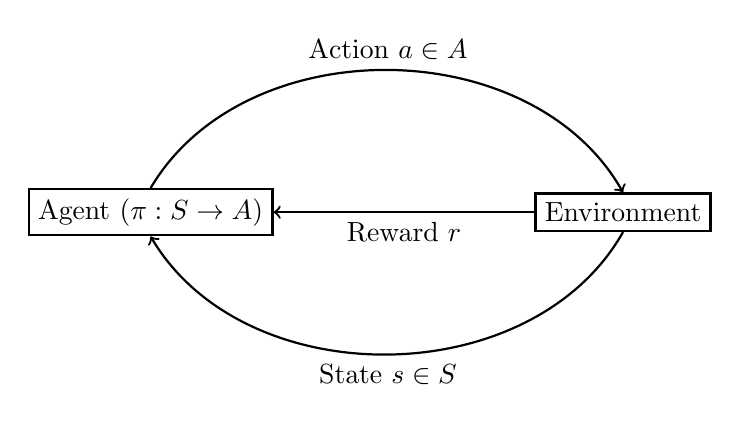
\begin{tikzpicture}[->, thick]
         %nodes
         \node[draw] at (-3,0) (agent) {Agent ($\pi: S \to A$)};
         \node[draw] at (3,0) (env) {Environment};
         \path
             (agent.north) edge[bend left=60] node[above] {Action $a \in A$} (env.north)
             (env.south) edge[bend left=60] node[below] {State $s \in S$} (agent.south)
             (env.west) edge node[below] {Reward $r$} (agent.east);
    \end{tikzpicture}
    \caption{The general reinforcement learning paradigm.}
    \label{fig:RL}
\end{figure}

% how RL can be applied to HE
% benefits of:
% fewer assumptions than AHT, could be more precise/better performance
% just specify target Hamiltonian and let algorithm learn
% specify experimental constraints
There are both potential benefits and drawbacks to using RL for Hamiltonian engineering. Approaches with average Hamiltonian theory require that pulse sequences be periodic and cyclic, approximate the propagator by using the lowest-order average Hamiltonian, and occasionally assume delta-function pulses. RL techniques would overcome these constraints and assumptions by calculating the propagator of a simulated quantum system numerically. This allows for non-periodic or acyclic pulse sequences to be considered, and accounts for finite pulse widths.
This may lead to novel pulse sequences that are more robust in experimental settings, where laboratory constraints (such as limited magnetic field strength or pulse timing) prevent the execution of ideal pulse sequences.
However, because RL techniques rely on simulated quantum systems to learn how to construct pulse sequences, there may be a discrepancy between performance on a small number of spins ($N=4$ spins in current simulation experiments) and performance in a laboratory setting with $\sim10^{23}$ spins. Furthermore, the typical issues associated with machine learning--lack of interpretability of results, no guarantees of convergence--are also associated with RL.

Several RL algorithms exist, each with different approaches depending on the nature of the state space $\mathcal{S}$ or action space $\mathcal{A}$. For Hamiltonian engineering, the action space is continuous: for each pulse, the axis of rotation, the field strength, and the duration can vary continuously (previous approaches to Hamiltonian engineering consider only a discrete set of actions for analytical tractability and to reduce to number of candidate pulse sequences). As a result, the deep deterministic policy gradient (DDPG) algorithm\cite{lillicrap2015continuous} was considered, but the hybrid algorithm Evolutionary Reinforcement Learning (ERL) \cite{khadka2018evolutionguided} was ultimately chosen.
DDPG is an actor-critic method, where the actor learns the deterministic policy $\pi: \mathcal{S} \to \mathcal{A}$ and the critic learns the action-value function $Q: \mathcal{S} \times \mathcal{A} \to \R$. The value $Q(s,a)$ returns the total expected future rewards by performing action $a$ while in state $s$. Neural network function approximators are used for both the policy $\pi$ and the action-value function $Q$. ERL implements DDPG alongside genetic algorithms to prevent premature convergence of the neural networks to local minima.

% state/action encoding
For a system of spin-1/2 particles, the \emph{actions} are magnetic field pulses that rotate the spins, and can therefore be parametrized by the axis of rotation, the rotation angle $\alpha$, and the time $dt$ over which the rotation is performed.
The axis of rotation is assumed to lie in the xy-plane, so a single pulse can be characterized by the tuple $(\phi, \alpha, dt) \in [-\pi,\pi] \times [-\alpha_\text{max}, \alpha_\text{max}] \times [t_\text{min}, \inf)$.
$\alpha_\text{max}$ and $t_\text{min}$ depend on the experimental limitations, but for this research the values $\alpha_\text{max} = 2\pi, t_\text{min} = 0$ were taken.
The relevant \emph{state} of the spin system is the propagator $U(t)$. However, the number of elements increases exponentially with the number of spins, so storing and computing with propagators quickly becomes infeasible.
Instead, the state is represented by the sequence of all previous actions performed. This contains the equivalent information stored in the propagator, and requires significantly less memory and computational power.

% fidelity, rewards
To quantify how well a given pulse sequence engineers the target Hamiltonian $H_\text{target}$, the following fidelity function is used:
\begin{equation}\label{eq:fidelity}
    \text{fidelity}(U_\text{target}^\dagger, U_\text{exp}) = \left| \text{Tr}\left( \frac{U_\text{target}^\dagger U_\text{exp}}{2^N} \right) \right|
\end{equation}
where $U_\text{target}$ is the propagator corresponding to $H_\text{target}$ over the length of the pulse sequence and $U_\text{exp}$ is the propagator corresponding to the pulse sequence itself. The fidelity is a scalar value between $0$ and $1$, with values closer to $1$ indicating better performance. Using this definition of fidelity, the rewards in the RL algorithm are
\begin{equation}\label{eq:rewards}
    r = -\log\left( 1- \text{fidelity}(U_\text{target}, U_\text{exp})^{\tau/t} \right)
\end{equation}
% TODO check that above is right
For short time intervals, both propagators $U_\text{target}$ and $U_\text{exp}$ are close to the identity, which would make the fidelity close to $1$. The exponent $\tau/t$ makes rewards comparable across different duration pulses sequences, decreasing fidelity for pulse sequence durations $t<\tau$ and increasing fidelity for $t>\tau$.

% network architecture
Neural network function approximators are used for both the actor's policy function and the critic's action-value function. The state and action inputs to the neural networks are individually mapped to the interval $[-1,1]$.
\begin{align}
    \phi \in [-\pi, \pi], \phi      &\mapsto \phi / \pi \\
    \alpha \in [-2\pi,2\pi],\alpha  &\mapsto \alpha / 2\pi \\
    t \in [0,5\cdot10^{-6}], t      &\mapsto
        \frac{\log_{10}(t + 10^{-7}) + 7}{0.853785} - 1
\end{align}
The actor's policy function is restricted to the values in the interval $[-1,1]$ via a tanh activation.
Because the state is represented by a sequence of actions, long short-term memory (LSTM) layers are used to process the state inputs\cite{lstm}. Fully connected layers with tanh and elu activation functions for the actor and critic respectively are used as hidden layers. See figure~\ref{fig:network-architecture} for a diagram of the network architectures.

\begin{figure}[ht]
    \centering
    % \includegraphics[width=0.7\linewidth]{graphics/epscor/network_architecture.jpeg}
    \begin{subfigure}{.49\textwidth}
        \centering
        % actor network
        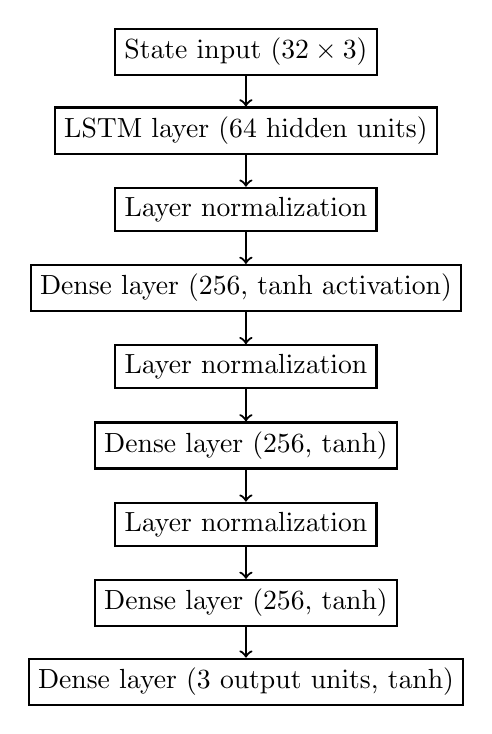
\begin{tikzpicture}[->, thick]
         %nodes
         \node[draw] at (0,5) (input) {State input ($32\times3$)};
         \node[draw] at (0,4) (lstm) {LSTM layer (64 hidden units)};
         \node[draw] at (0,3) (lnorm1) {Layer normalization};
         \node[draw] at (0,2) (d1) {Dense layer (256, tanh activation)};
         \node[draw] at (0,1) (lnorm2) {Layer normalization};
         \node[draw] at (0,0) (d2) {Dense layer (256, tanh)};
         \node[draw] at (0,-1) (lnorm3) {Layer normalization};
         \node[draw] at (0,-2) (d3) {Dense layer (256, tanh)};
         \node[draw] at (0,-3) (output) {Dense layer (3 output units, tanh)};
         % arrows between nodes
         \draw (input) -- (lstm); \draw (lstm) -- (lnorm1);
         \draw (lnorm1)--(d1); \draw(d1)--(lnorm2); \draw (lnorm2) -- (d2);
         \draw (d2) -- (lnorm3); \draw (lnorm3) -- (d3); \draw (d3) -- (output);
        \end{tikzpicture}
        \caption{The actor neural network to learn the policy $\pi(s)$.}
    \end{subfigure}
    \begin{subfigure}{.49\textwidth}
        \centering
        % critic network
        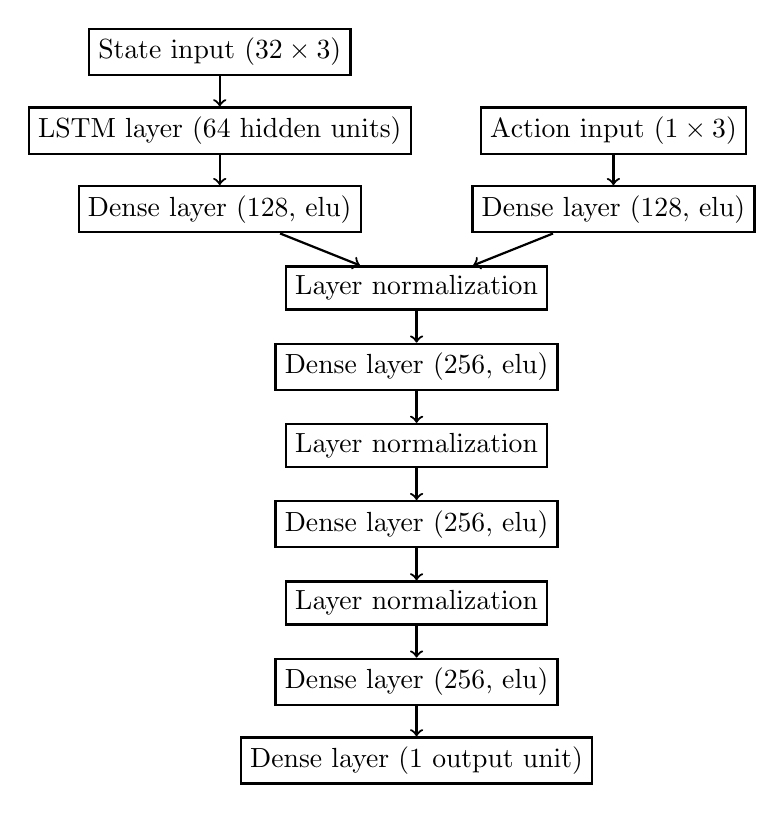
\begin{tikzpicture}[->, thick]
         %nodes
         \node[draw] at (-2.5,4) (sinput) {State input ($32\times3$)};
         \node[draw] at (-2.5,3) (lstm) {LSTM layer (64 hidden units)};
         \node[draw] at (-2.5,2) (d1a) {Dense layer (128, elu)};
         \node[draw] at (2.5,3) (ainput) {Action input ($1\times 3$)};
         \node[draw] at (2.5,2) (d1b) {Dense layer (128, elu)};
         \node[draw] at (0,1) (lnorm1) {Layer normalization};
         \node[draw] at (0,0) (d2) {Dense layer (256, elu)};
         \node[draw] at (0,-1) (lnorm2) {Layer normalization};
         \node[draw] at (0,-2) (d3) {Dense layer (256, elu)};
         \node[draw] at (0,-3) (lnorm3) {Layer normalization};
         \node[draw] at (0,-4) (d4) {Dense layer (256, elu)};
         \node[draw] at (0,-5) (output) {Dense layer (1 output unit)};
         % arrows between nodes
         \draw (sinput) -- (lstm); \draw (lstm) -- (d1a);
         \draw (ainput) -- (d1b); \draw(d1a)--(lnorm1); \draw(d1b)--(lnorm1);
         \draw (lnorm1)--(d2); \draw (d2) -- (lnorm2);
         \draw (lnorm2) -- (d3); \draw (d3) -- (lnorm3); \draw (lnorm3) -- (d4);
         \draw (d4) -- (output);
        \end{tikzpicture}
        \caption{The critic neural network to learn $Q(s,a)$.}
    \end{subfigure}
    \caption{Neural network architectures .}
    \label{fig:network-architecture}
\end{figure}


Preliminary results using ERL for pulse sequence design indicate worse performance than existing Hamiltonian engineering methods, but many modifications to the algorithm remain to be explored.
The policy-gradient actor does not improve its performance over time, and the evolution-guided population of actors also does not improve (see figure~\ref{fig:results}). The lack of improvement in the population is understandable, because any change in policy is from random mutations to the neural network weights. The policy-gradient actor performs gradient ascent using the critic's $Q$ function, so it is likely that the critic is not effectively learning state-action values.
% preliminary results
\begin{figure}[ht]
    \centering
    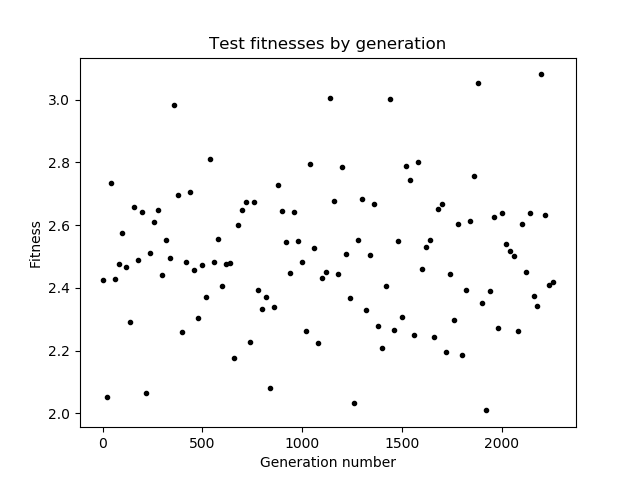
\includegraphics[width=0.7\linewidth]{graphics/test_fit.png}
    \caption{The fitnesses (i.e. the maximum reward in the episode) of the highest-fitness actor by generation.}
    \label{fig:results}
\end{figure}
% compare to existing methods, NEXT STEPS
The poor performance may be due to poor choice of hyperparameters (such as the learning rate or the number of observations from which to learn) or ineffective exploration of both state and action space.
% TODO talk about null action as local minima already, small
% deviations away from 0 are lower rewards
% TODO also possibility of discrete actions/stochastic policy
Further work is needed to explore both of these possibilities.

\printbibliography

\end{document}
